
\documentclass[11pt]{article}
\usepackage[margin=1in]{geometry}
\usepackage{amsmath,amssymb,booktabs,array,longtable}
\usepackage{graphicx}
\usepackage{hyperref}
\usepackage{enumitem}
\usepackage{titlesec}

\begin{document}

\begin{center}
\Large\textbf{Shiv Nadar University Chennai}\\[2mm]
\end{center}

\renewcommand{\arraystretch}{1.4}

\begin{tabular}{|p{3.5cm}|p{8cm}|p{2cm}|}
\hline
Degree \& Branch & B.Tech Artificial Intelligence \& Data Science & Semester V\\ \hline
Subject Code \& Name & CS3807 -- Deep Learning Laboratory & AY: 2026--27\\ \hline
\end{tabular}

\vspace{3mm}

\begin{center}
\Large\textbf{Experiment 1}\\
\large\textbf{Implementation of a Single Layer Perceptron for Binary Classification}
\end{center}

%----------------------------------------------------------

\section*{1. Objective}

The objective of this experiment is to understand the concept of an artificial neuron and implement a Single Layer Perceptron from scratch for binary classification. Students will learn the perceptron learning algorithm, understand the importance of activation functions, visualize the learning process, and evaluate the classifier using a real-world dataset.

%----------------------------------------------------------

\section*{2. Background Theory}

An Artificial Neuron is the fundamental building block of a neural network. It receives one or more input features, multiplies them by corresponding weights, adds a bias term, and applies an activation function to determine the output.

The Single Layer Perceptron is the earliest supervised learning algorithm capable of solving linearly separable binary classification problems.

\subsection*{Mathematical Formulation}

Weighted Sum

\[
z=\mathbf{w}^{T}\mathbf{x}+b
\]

where

\begin{itemize}
\item $\mathbf{x}$ : Input vector
\item $\mathbf{w}$ : Weight vector
\item $b$ : Bias
\item $z$ : Linear combination
\end{itemize}

Prediction

\[
\hat y=f(z)
\]

Weight Update Rule

\[
\mathbf{w}_{new}
=
\mathbf{w}_{old}
+
\eta
(y-\hat y)
\mathbf{x}
\]

Bias Update

\[
b_{new}
=
b_{old}
+
\eta
(y-\hat y)
\]

where $\eta$ denotes the learning rate.

%----------------------------------------------------------

\section*{3. Activation Functions}

An activation function determines the output of a neuron based on the weighted sum of its inputs. It introduces non-linearity, enabling neural networks to learn complex patterns. Although the perceptron uses only the Step Activation Function, modern deep learning models employ differentiable activation functions for efficient optimization through backpropagation.

\subsection*{Step Activation Function}

\[
f(z)=
\begin{cases}
1,&z\ge0\\
0,&z<0
\end{cases}
\]

The Step Activation Function produces a binary output and is therefore suitable only for linearly separable binary classification problems.

\begin{center}
\begin{tabular}{|p{2.5cm}|p{3cm}|p{6cm}|}
\hline
\textbf{Activation} & \textbf{Output Range} & \textbf{Typical Applications}\\
\hline
Step & $\{0,1\}$ & Classical Perceptron\\
\hline
Sigmoid & $(0,1)$ & Binary Classification Output Layer\\
\hline
Tanh & $(-1,1)$ & Hidden Layers (Traditional Networks)\\
\hline
ReLU & $[0,\infty)$ & Hidden Layers in CNNs and MLPs\\
\hline
Leaky ReLU & $(-\infty,\infty)$ & Avoiding Dying ReLU\\
\hline
Softmax & $(0,1)$ & Multi-class Classification Output Layer\\
\hline
\end{tabular}
\end{center}

\textbf{Note:} This experiment uses only the Step Activation Function. The remaining activation functions will be studied in subsequent experiments involving Multilayer Perceptrons and Deep Neural Networks.

%----------------------------------------------------------

\section*{4. Dataset Description}

\textbf{Dataset:} Banknote Authentication Dataset

\textbf{Source:} UCI Machine Learning Repository

\textbf{Download Link:}

\url{https://archive.ics.uci.edu/dataset/267/banknote+authentication}

\begin{center}
\begin{tabular}{|l|l|}
\hline
Instances & 1372\\
\hline
Features & 4 Numerical Features\\
\hline
Classes & 2\\
\hline
Missing Values & None\\
\hline
Task & Binary Classification\\
\hline
\end{tabular}
\end{center}

\textbf{Feature Description}

\begin{itemize}
\item Variance
\item Skewness
\item Curtosis
\item Entropy
\end{itemize}

Target Class

\begin{itemize}
\item 0 -- Authentic Banknote
\item 1 -- Forged Banknote
\end{itemize}

%----------------------------------------------------------

\section*{5. Source Code}

The complete source code for this experiment, including dataset loading, exploratory data analysis, the from-scratch Single Layer Perceptron implementation, training, evaluation, and all plot generation, is available at the following GitHub repository:

\begin{center}
\url{https://github.com/UvanAdhithya/DeepLearning-Lab}
\end{center}

%----------------------------------------------------------

\section*{6. Mandatory Plots}

\subsection*{Feature Histograms, Correlation Heatmap, Scatter Plot and Boxplots}

\begin{center}
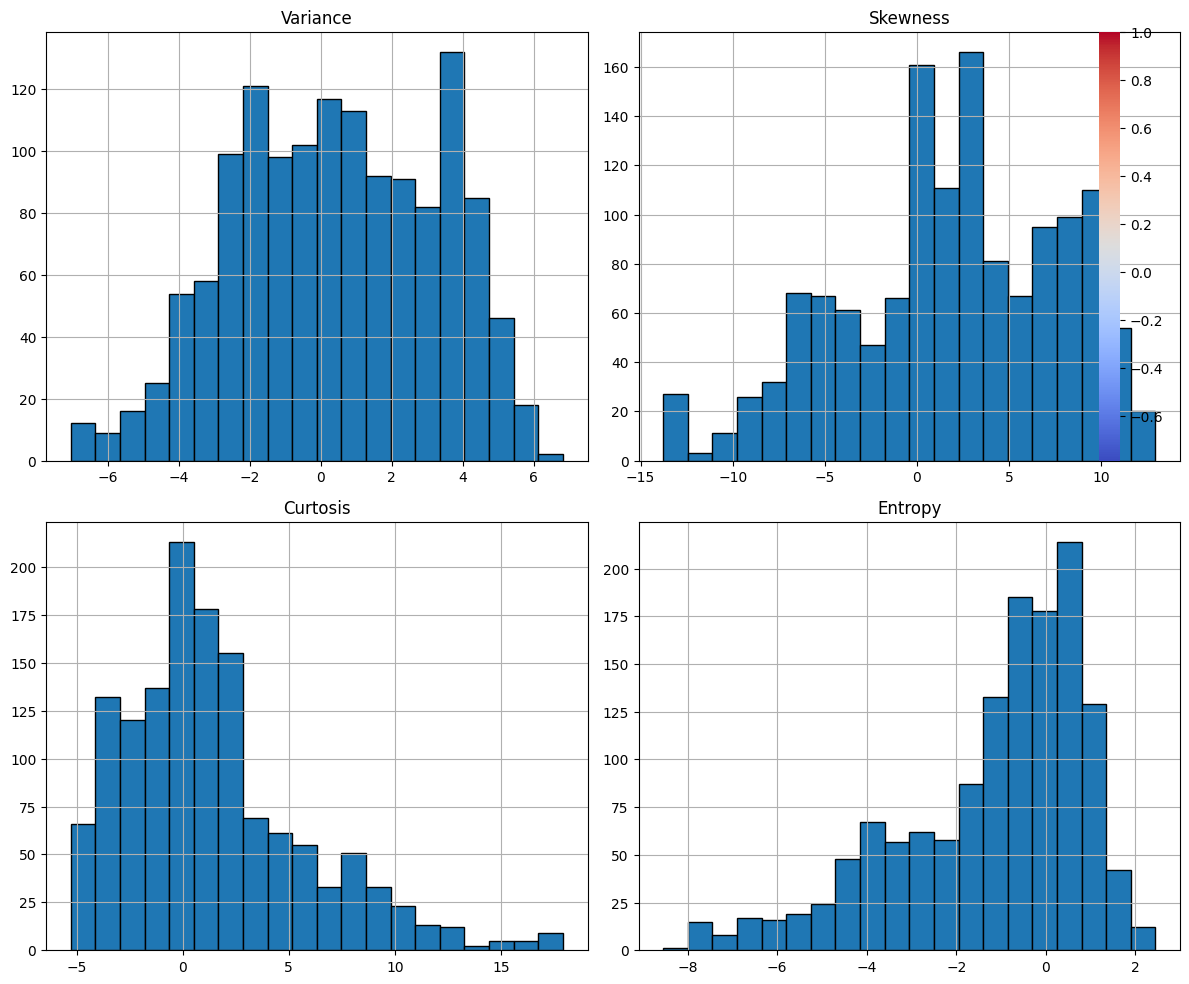
\includegraphics[width=0.95\textwidth]{eda_fig.png}
\end{center}

As we can see in the histograms, the distributions of Variance and Entropy are fairly symmetric, while the distributions of both Skewness and Curtosis appear to be heavily right-skewed, with Curtosis having the most extreme outliers. From the correlation heatmap, we can easily see there is a strong negative correlation between Variance and Class and we can also see there is a somewhat strong negative correlation between Skewness and Curtosis. From the scatter plot of Variance against Skewness, we can observe that the two classes are almost but not completely linearly separable. The boxplots suggest, once again, that the variability in Skewness and Curtosis is higher than the variability of the other two features.
\vspace{4mm}

\subsection*{Training Error vs Epoch, Weight Evolution, Bias Evolution and Confusion Matrix}

\begin{center}
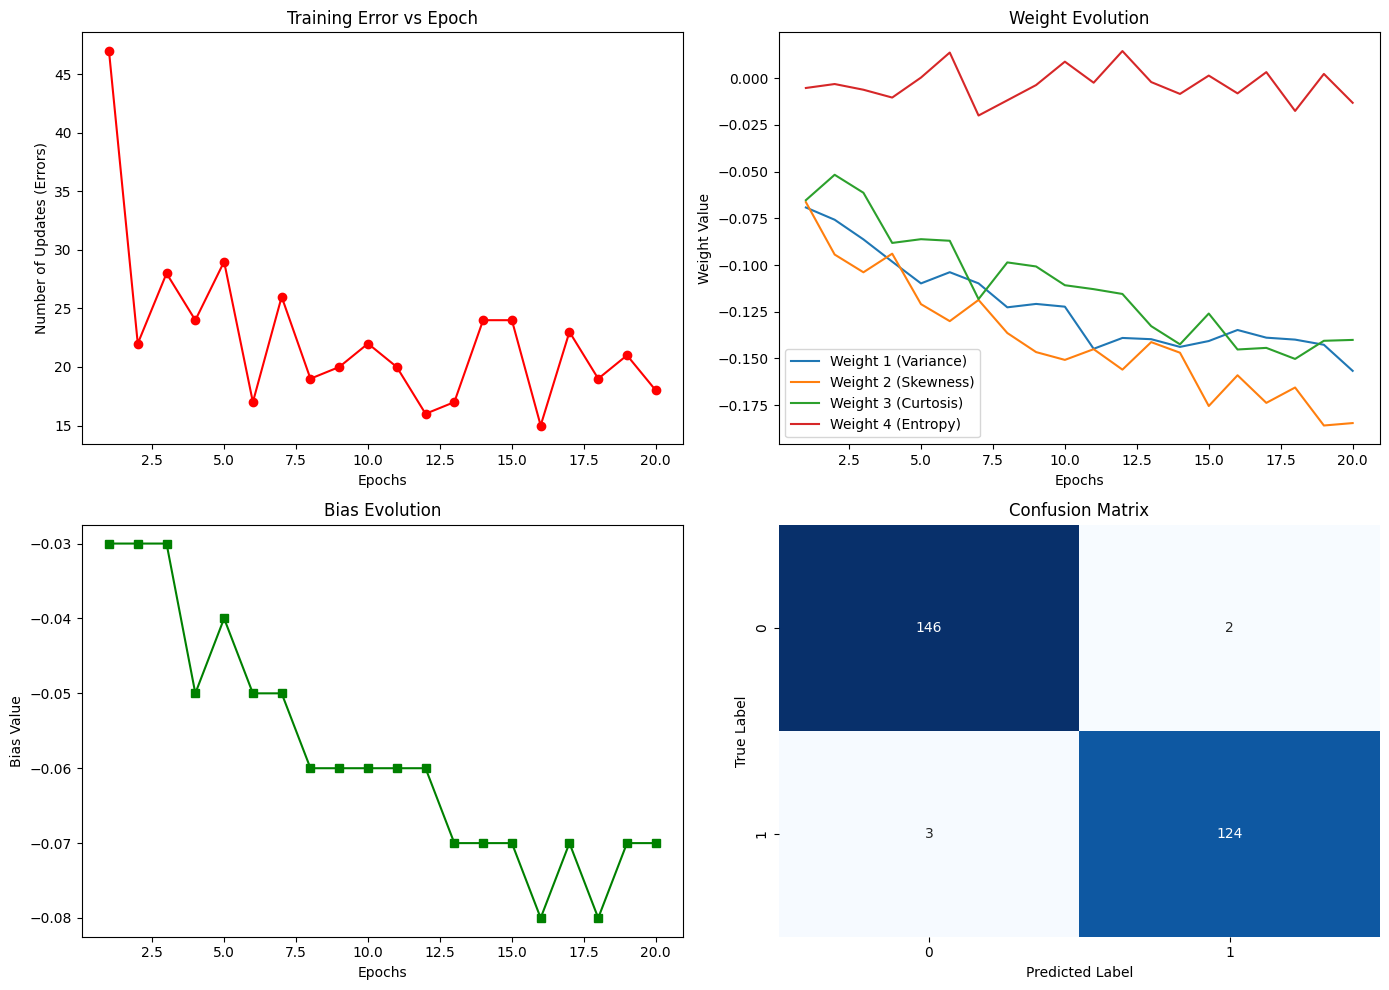
\includegraphics[width=0.95\textwidth]{task7_fig.png}
\end{center}

The Training Error vs Epoch graph demonstrates that the number of misclassifications has dropped sharply from 47 to 22 during the first two epochs, before steadily oscillating between 15 and 29, which implies that the classes are not completely linearly separable. The Weight Evolution graph demonstrates that Variance's and Skewness' weights decline and stabilize at roughly $-0.15$ to $-0.18$. The Bias Evolution graph indicates that the bias drifts downward stepwise from $-0.03$ to $-0.07$. The Confusion Matrix confirms only 2 false positives and 3 false negatives for the 275 test samples examined.

\vspace{4mm}

\subsection*{Learning Rate Comparison}

\begin{center}
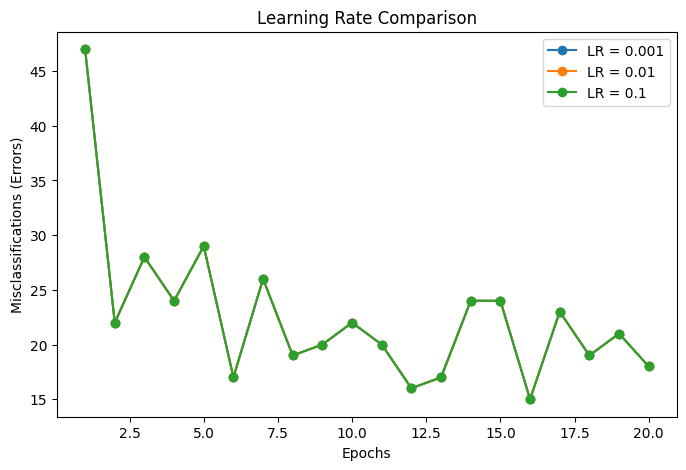
\includegraphics[width=0.7\textwidth]{lr_comparison.png}
\end{center}

The misclassification curves for learning rates of 0.001, 0.01, and 0.1 are almost identical as all weight updates (and hence predictions at each and every step) follow the same sign in the case of zero initialized weights and only differ in magnitude with $\eta$. This means that for the given dataset, the convergence behavior of the perceptron (the number of epochs required for stabilization, the trend of oscillation behavior, etc.) remains unaffected from the learning rate but differs in only the final magnitude of weights.

\vspace{4mm}

\subsection*{Decision Boundary (Optional)}

\begin{center}
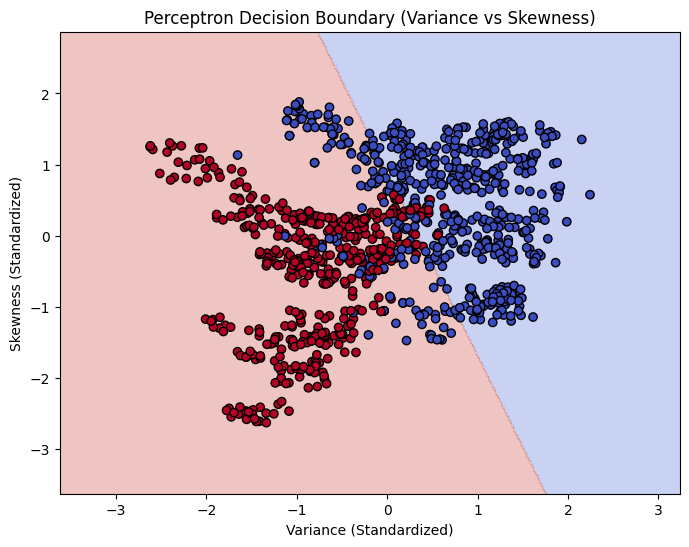
\includegraphics[width=0.7\textwidth]{decision_boundary.png}
\end{center}

By using only the Variance and Skewness features, the perceptron is able to form a straight line that distinguishes the majority of real (blue) banknotes from counterfeit (red) ones. It has been proven that the higher the Variance, the greater the chance of being a real banknote. The band of misclassified points visible close to the separating line confirms that the two features are not totally linearly separable.

%----------------------------------------------------------

\section*{7. Performance Tables}

\textbf{Training Summary}

\begin{tabular}{|p{6cm}|p{7cm}|}
\hline
Dataset Size & 1372 samples\\
\hline
Train/Test Split & 1097 / 275 (80\% / 20\%)\\
\hline
Learning Rate & 0.01\\
\hline
Epochs & 20\\
\hline
Final Weights & [-0.1567, -0.1846, -0.1401, -0.0132]\\
\hline
Final Bias & -0.0700\\
\hline
Accuracy & 0.9818\\
\hline
Precision & 0.9841\\
\hline
Recall & 0.9764\\
\hline
F1-score & 0.9802\\
\hline
\end{tabular}

\vspace{3mm}

\textbf{Epoch-wise Learning} (Variance and Skewness weights shown; $\eta = 0.01$)

\begin{tabular}{|c|c|c|c|c|}
\hline
Epoch & Errors & Weight 1 (Variance) & Weight 2 (Skewness) & Bias\\
\hline
1 & 47 & -0.0692 & -0.0663 & -0.0300\\
2 & 22 & -0.0758 & -0.0944 & -0.0300\\
3 & 28 & -0.0863 & -0.1039 & -0.0300\\
4 & 24 & -0.0982 & -0.0939 & -0.0500\\
5 & 29 & -0.1098 & -0.1210 & -0.0400\\
$\vdots$ & $\vdots$ & $\vdots$ & $\vdots$ & $\vdots$\\
16 & 15 & -0.1348 & -0.1590 & -0.0800\\
17 & 23 & -0.1389 & -0.1738 & -0.0700\\
18 & 19 & -0.1399 & -0.1656 & -0.0800\\
19 & 21 & -0.1427 & -0.1859 & -0.0700\\
20 & 18 & -0.1567 & -0.1846 & -0.0700\\
\hline
\end{tabular}

%----------------------------------------------------------

\section*{8. Discussion and Conclusion}

A fully trained Single Layer Perceptron using the Banknote Authentication dataset showed impressive performance with the test accuracy of 98.18 % when ratioed with precision, recall and F1 values exceeding 0.97. Since this confirms the linear separability of the two classes represented with four features (Variance, Skewness, Curtosis and Entropy), the training error during 20 epochs did not go down to zero as it ranged from 15 to 29 errors every epoch after the initial drop, which means that only a small number of samples were mistakenly classified. Furthermore, comparing the learning rates demonstrated that the learning rate had no effect on the rates of misclassification during the training for this zero-initiated perceptron because its only function is scaling the magnitude of weight corrections. Eventually, upon utilizing decision boundaries with only two features (Variance and Skewness), the network still performed well but with the noticeable overlap in the area of boundary that confirms the importance of using Curtosis and Entropy in the classification The custom implementation's accuracy (98.18\%) was very close to that of Scikit-learn's built-in Perceptron (98.55\%), validating the correctness of the from-scratch implementation of the weighted sum, step activation, and the perceptron learning rule. Overall, the experiment demonstrates both the strengths of the perceptron as a simple, interpretable linear classifier on well-behaved data, and its fundamental limitation on data that is not perfectly linearly separable.

%----------------------------------------------------------

\section*{9. References}

\begin{enumerate}
\item F. Rosenblatt, ``The Perceptron,'' \emph{Psychological Review}, 1958.
\item I. Goodfellow, Y. Bengio and A. Courville, \emph{Deep Learning}, MIT Press, 2016.
\item C. M. Bishop, \emph{Pattern Recognition and Machine Learning}, Springer, 2006.
\item S. Haykin, \emph{Neural Networks and Learning Machines}, Pearson, 2009.
\item UCI Machine Learning Repository -- Banknote Authentication Dataset.
\item Scikit-learn Documentation: Perceptron.
\end{enumerate}

\end{document}

